\chapter{clustering}
 
\section{DBSCAN}
\theoremstyle{plain}
The key idea of density-based clustering \cite{Ester96adensity} is that for each 		\cite{Mendes:2011:DSS:2063518.2063519}
object of a cluster the neighborhood of a given radius $\epsilon$ (Eps)
has to contain at least a minimum number of objects
(MinPts), i.e. the cardinality of the neighborhood has to exceed
some threshold.
We will first give a short introduction to DBSCAN including
the definitions which are required for incremental 
clustering.
%defizioni di DBSCAN
\begin{definizione}[directly density-reachable]
\label{def:ddr}
Un oggetto $p$ si dice 	"\emph{directly-density-reachable}" da un oggetto $q$ wrt $Eps$ ed $MinPts$ nell'insieme di oggetti $D$ se:
\begin{enumerate}
\item $p \in N_{eps(Q)}$
\item $|N_{eps(Q)}| \ge MinPts$
\end{enumerate}
\end{definizione}
\begin{definizione}[density-reachable]
\label{def:dr} 
Un oggetto   $p$ si dice 	\emph{"density-reachable"} da un oggetto $q$ wrt $Eps$ ed $MinPts$ nell'insieme di oggetti $D$, e si  indica con \emph{$p>_{D}q$}, se esiste una catena di oggetti: $p_1,\dots,p_n$, $p_1=p p_n=q$ tali che:  $p_{i} \in D  \land p_{i+1}$ è \emph{directly-density-reachable} da $p_{i}$
Questa relazione è l'estensione canonica della relazione Directly-density-reachability, inoltre è una relaione transitiva ma non simmetrica. Sebbene non sia simmetrica, vi sono delle zone nell'isnieme $D$, in cui questa relazione è simmetrica ovvero  per quegli oggetti $o$ nell insieme per cui $|N_{eps(o)}| \ge MinPts$. Due oggetti \emph{border}, ovvero due oggetti che giacciono sul confine di un cluser, probabilmente non saranno density-reachable fra loro in quanto non ci sono abbastanza oggetti nel loro vicinato. Tuttavia, ci sarà necessariamente, un terzo oggetto nel cluster dal quale entrambi questi  oggetti border saranno density-reachable.
\end{definizione}
%figura esempio
\begin{figure}
%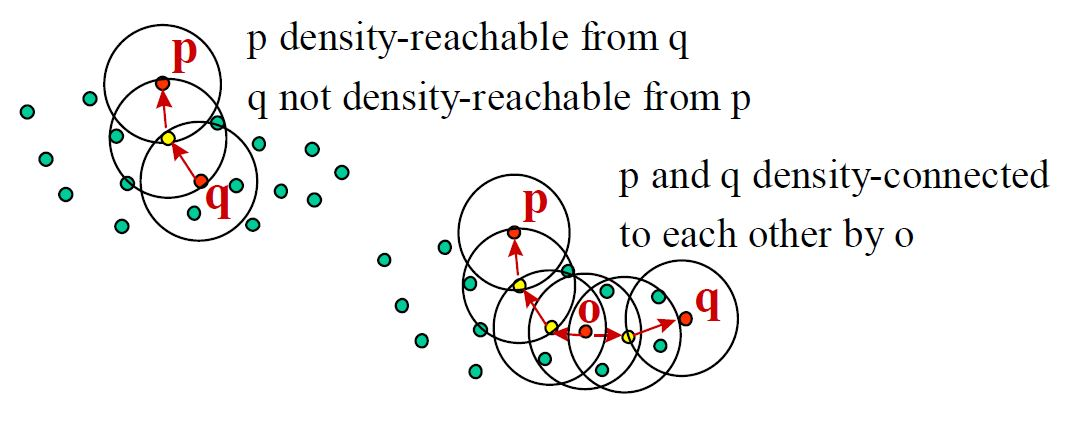
\includegraphics[scale=0.5]{images/density-reachable}
\caption{Density Reachability e Density Connectivity}
\label{fig:dens-reach}
\end{figure}
%density connected def
\begin{definizione}[density-connected]
\label{def:dc}
Un oggetto $p$ si dice 	\emph{"density-connected"} da un oggetto $q$ wrt $Eps$ ed $MinPts$ nell'insieme di oggetti $D$ se esiste un oggetto $o \in D$  tale che sia $p$ che $q$ siano \emph{ density reachable} da $o$. La relazione di density-connectivity è simmetrica, la figura \ref{fig:dens-reach} mostra la le definizioni su descritte in uno spazio bi-dimensionale. 
\end{definizione} 
Proprio grazie alla proprietà di density connectivity, si potrà dare la definizione di cluster ovvero un insieme massimale di oggetti \emph{"density-connected"}.
%cluster def
\begin{definizione}[cluster]
\label{def:cluster}
Sia $D$ un insieme di oggetti.
Si defnisce \emph{"cluster"}  $C$,  wrt $Eps$ ed $MinPts$ nell'insieme di oggetti $D$,
un sottoniseme non vuoto di $D$, che soddisfa le seguenti condizioni :
\begin{enumerate}
\item \emph{Massimalità}: $\forall p,q\in D$, se $p \in C \land q>_{D}p$ wrt MinPts e Eps, 
allora anche $q \in C  $

\item \emph{Connettività}: $\forall p,q\in C$, $p$ è \emph{"density-connected"} a $q$  wrt MinPts e Eps

\end{enumerate}
 
\end{definizione} 


%def noise
\begin{definizione}[noise]
\label{def:noise}
Siano $C_1,\dots,C_k$ tutti i cluster wrt Eps e MinPts in $D$. Si definisce \emph{noise}  l'insieme di oggetti $D$ che non appartengono a nessun cluster $C_i$,
noise=$\lbrace p\in D | \forall i: p \notin C_i \rbrace $.
 
\end{definizione}
Esistono due tipologie di oggetti nel clustering \emph{core-objects} sono quegli oggetti che soddisfano la seconda condizione della definizione \ref{def:ddr}, (ovvero che hanno un viciniato molto denso), e non \emph{non-core-objects} che non rispettano la condizione. I \emph{non-core-objects} possono essere sia oggetti \emph{border-objects} (oggetti non core, ma che sono \emph{density-reachable} da un \emph{core-object}
 
 





